\section{Planning phase}
	In this section it will be described how the project startet
	and how the project was defined with scope and requirements.

\subsection{Getting to know each other and the customer}
	At the kickoff of the project, the groups and the customer did not know 
	each other. The fist thing the course staff did was to set all the groups
	together and introduce them to the customer. 

	After the introduction to the course, the students sat down and talked while
	all the customers had a lunch. Later that they, all the groups had a meeting 
	with the customer. At this meeting, the group and the students, sat down and 
	the customer talked about their company. When the students knew some more about
	the customer, the project and the requirements was in focus. 

	In the end of the meeting, the customer wanted the students to come up
	with a game concept and a requirement specification. 
	

\subsection{Project Assignment}
	Before the project started the group got a description of the problem
	in the compendium that was handed out to the course memembers. The 
	description from Helgelandskraft was: 
		\paragraph{Power Control Game}
		{\it The idea is to make a casual game for mobile devices focused around controlling 
		power production from hydro plants trough a power grid to large industry customers and 
		regular consumers, or some other casual game involving power grids, hydro plants 
		and/or other themes around hydro power. 
		 
		The application should also provide the user with power preservation tips, like a 
		tip on loading screens or the splash screen when opening the game. Tips like: 
		 
		“19-21 degrees celsius is a good inside temperature. For each degree you lower the temperature 
		you’ll save 5 procent of the energy used for heating up your living space. 
		You can lower the temperature even more in rooms you normally don’t use.” 
		 
		The application should be developed for iOS and Android. We’ll provide the 
		students with the required equipment needed for iOS-development if they don’t 
		have it, and an android phone if they need it. 
		 
		The application should be designed for the tips and the language to easily be changed.}

	Helgelandskraft wanted a game running on android and Ios, with main theme "power".
	In the project description they introduced some key points, but they did not have a
	concrete idea of what they realy wanted. The scoping of the project and the developing
	of the game project was the next phase to do.

\subsection{Define the Project Scope}


\subsection{Preliminary studies and Project Planning}
	Before starting the project, we needed to do some reseach on project methodology, 
	game concepts and technology. This was a important phase since this type of 
	project was new to the students. 

	\begin{figure}[H]
		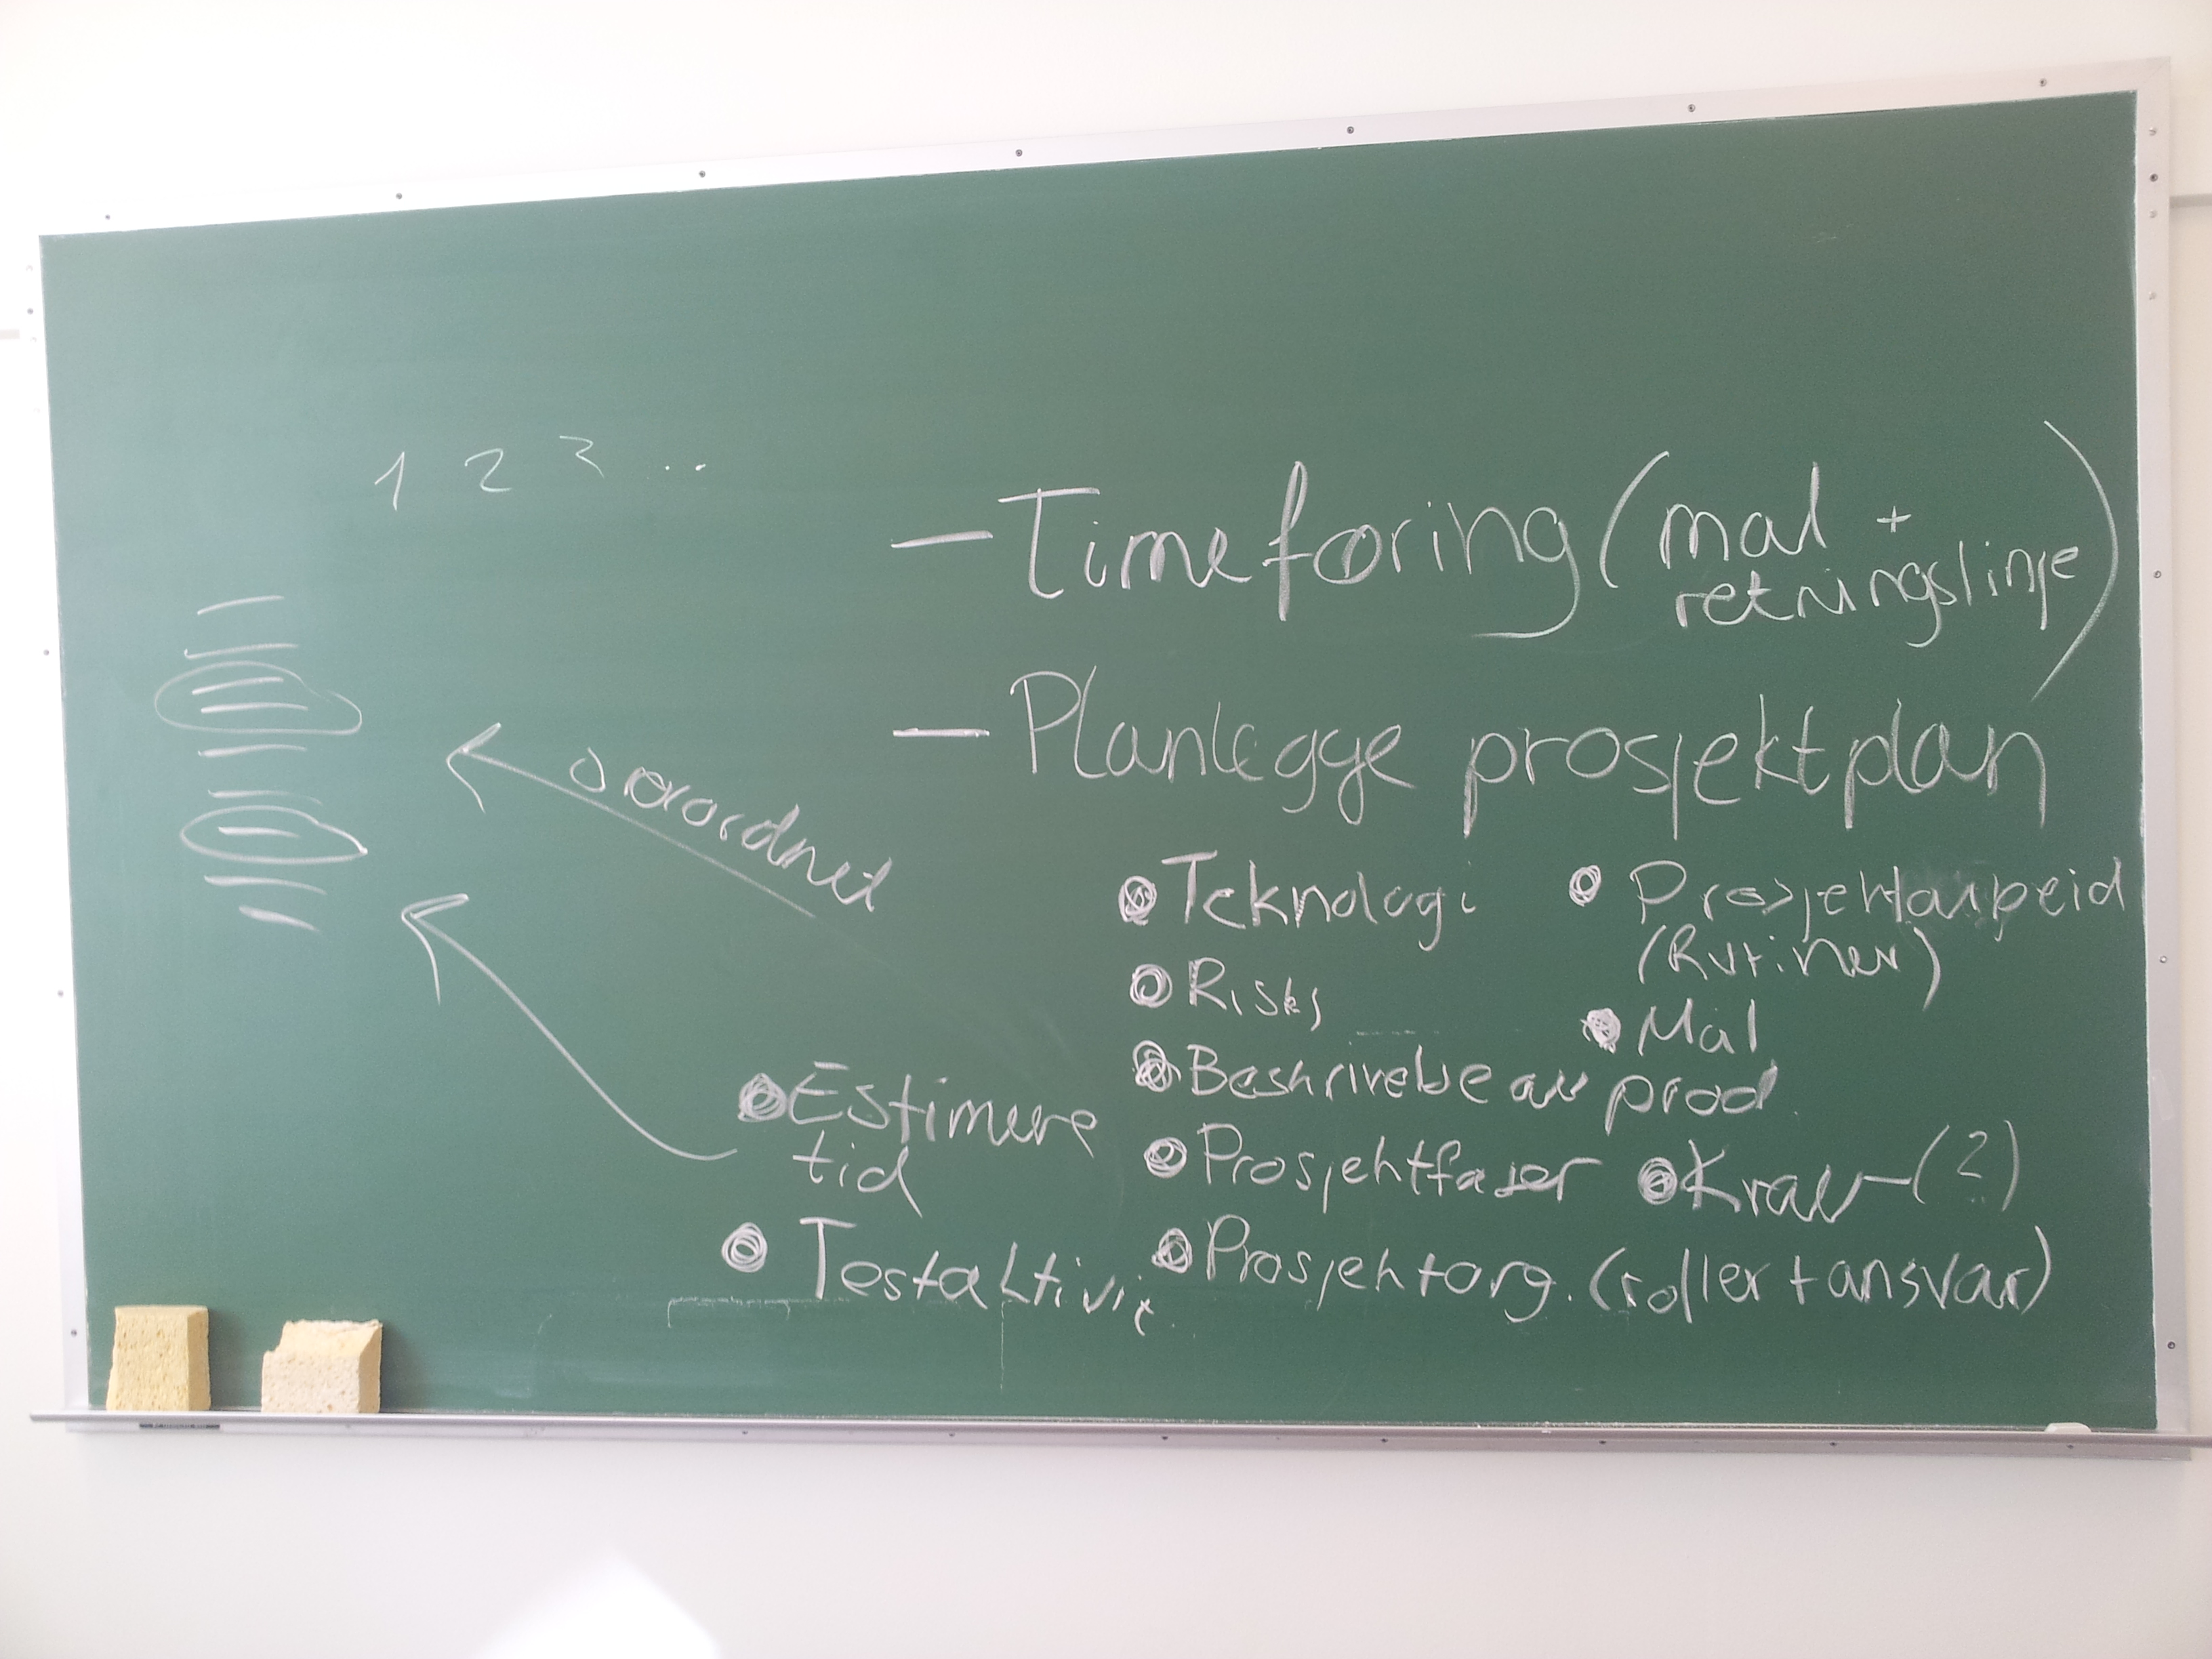
\includegraphics[scale=0.10]{pictures/projectPlanning.jpg}
	\end{figure}

\subsection{Game Concept Development}
	The customer did not know what they wanted the students to deliver in the end of 
	this project. The only thing they knew was that they wanted a power-game that
	was running on android and Ios. 

	The group sat down in a "green zone". The green zone concept is that each team member
	is sitting 10 minutes alone and try to coming up with a concept. After the 10 minutes
	all the members presents their ideas to the rest of the team members.
	After presenting all the consepts, the grpup picked out the best ideas. 

	The first concept was a "shortest-path-problem" game where the player should
	connect a number of nodes with lines without crossing the lines. The goal 
	wad to get the shortest path between the nodes. When the group presented this
	to the customer, they liked the idea, but they wanted a more "real life" game.

	The next concept was a "sim city" like concept, and is the game concept that
	we chose do implement. A description of this can you find in the "Game Concept"
	section. 

	\begin{figure}[H]
	\centering
		\subfigure{
			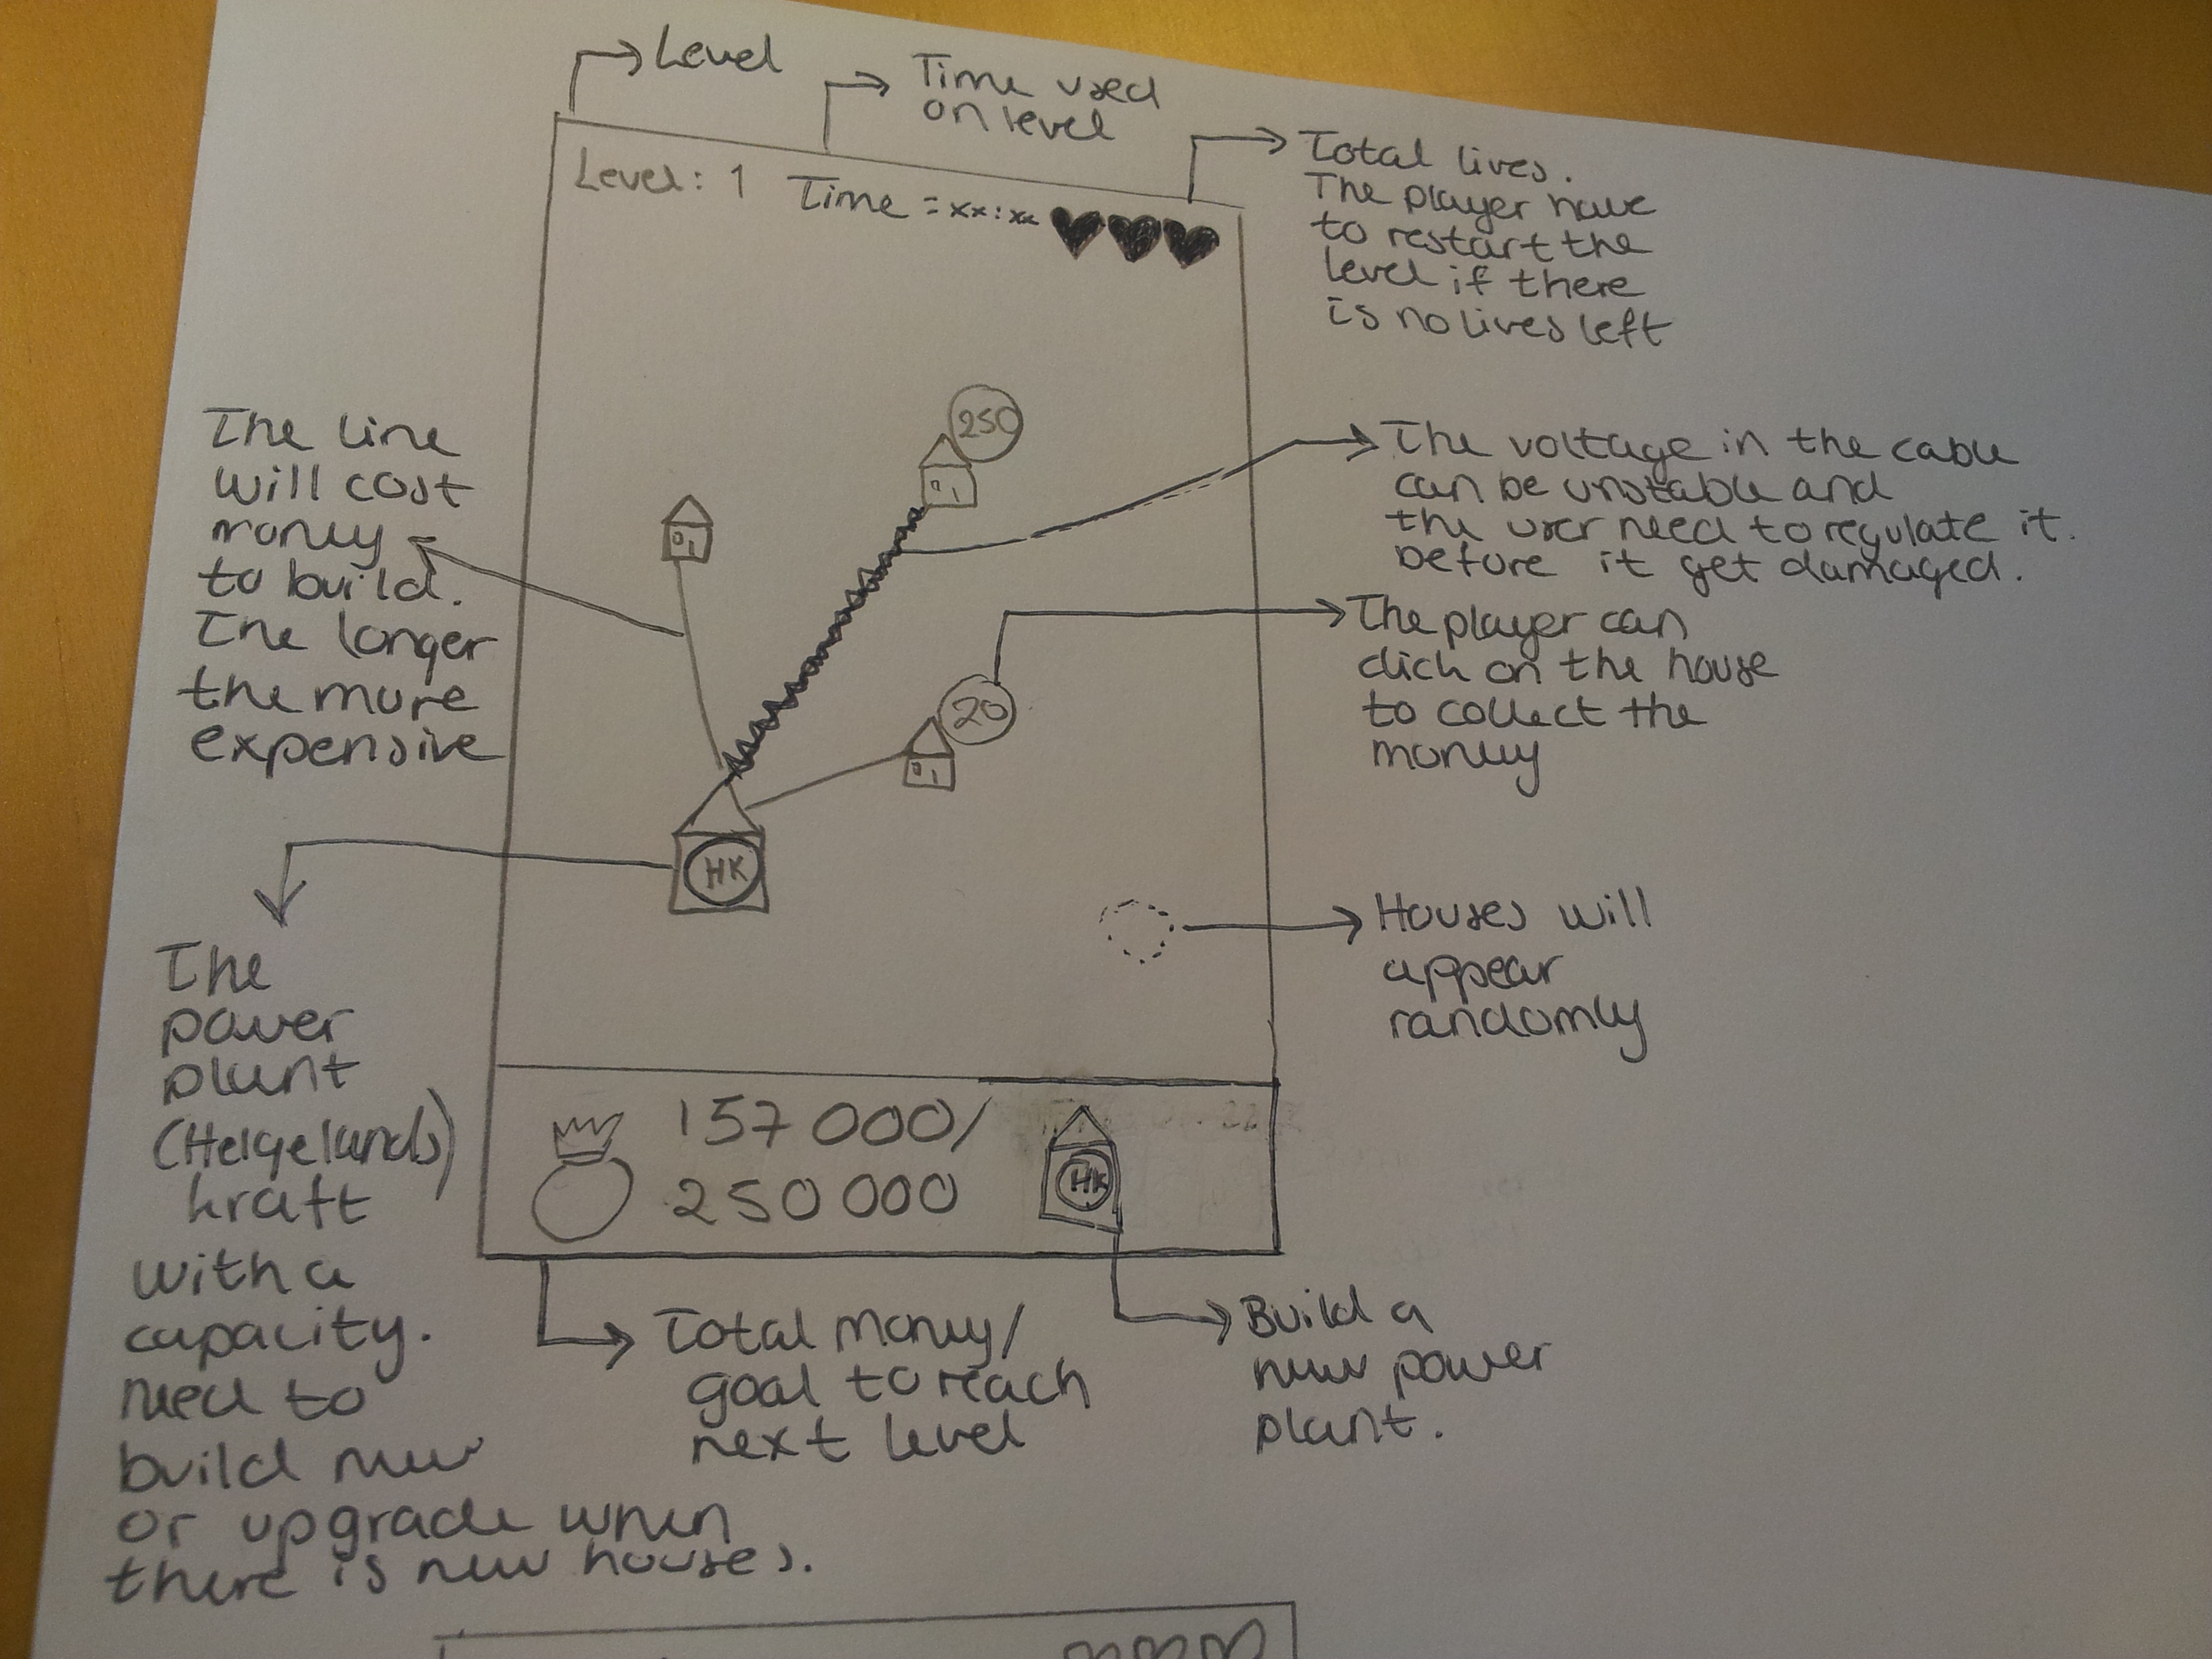
\includegraphics[scale=0.05]{pictures/gameConcept1}
		}
		\subfigure{
			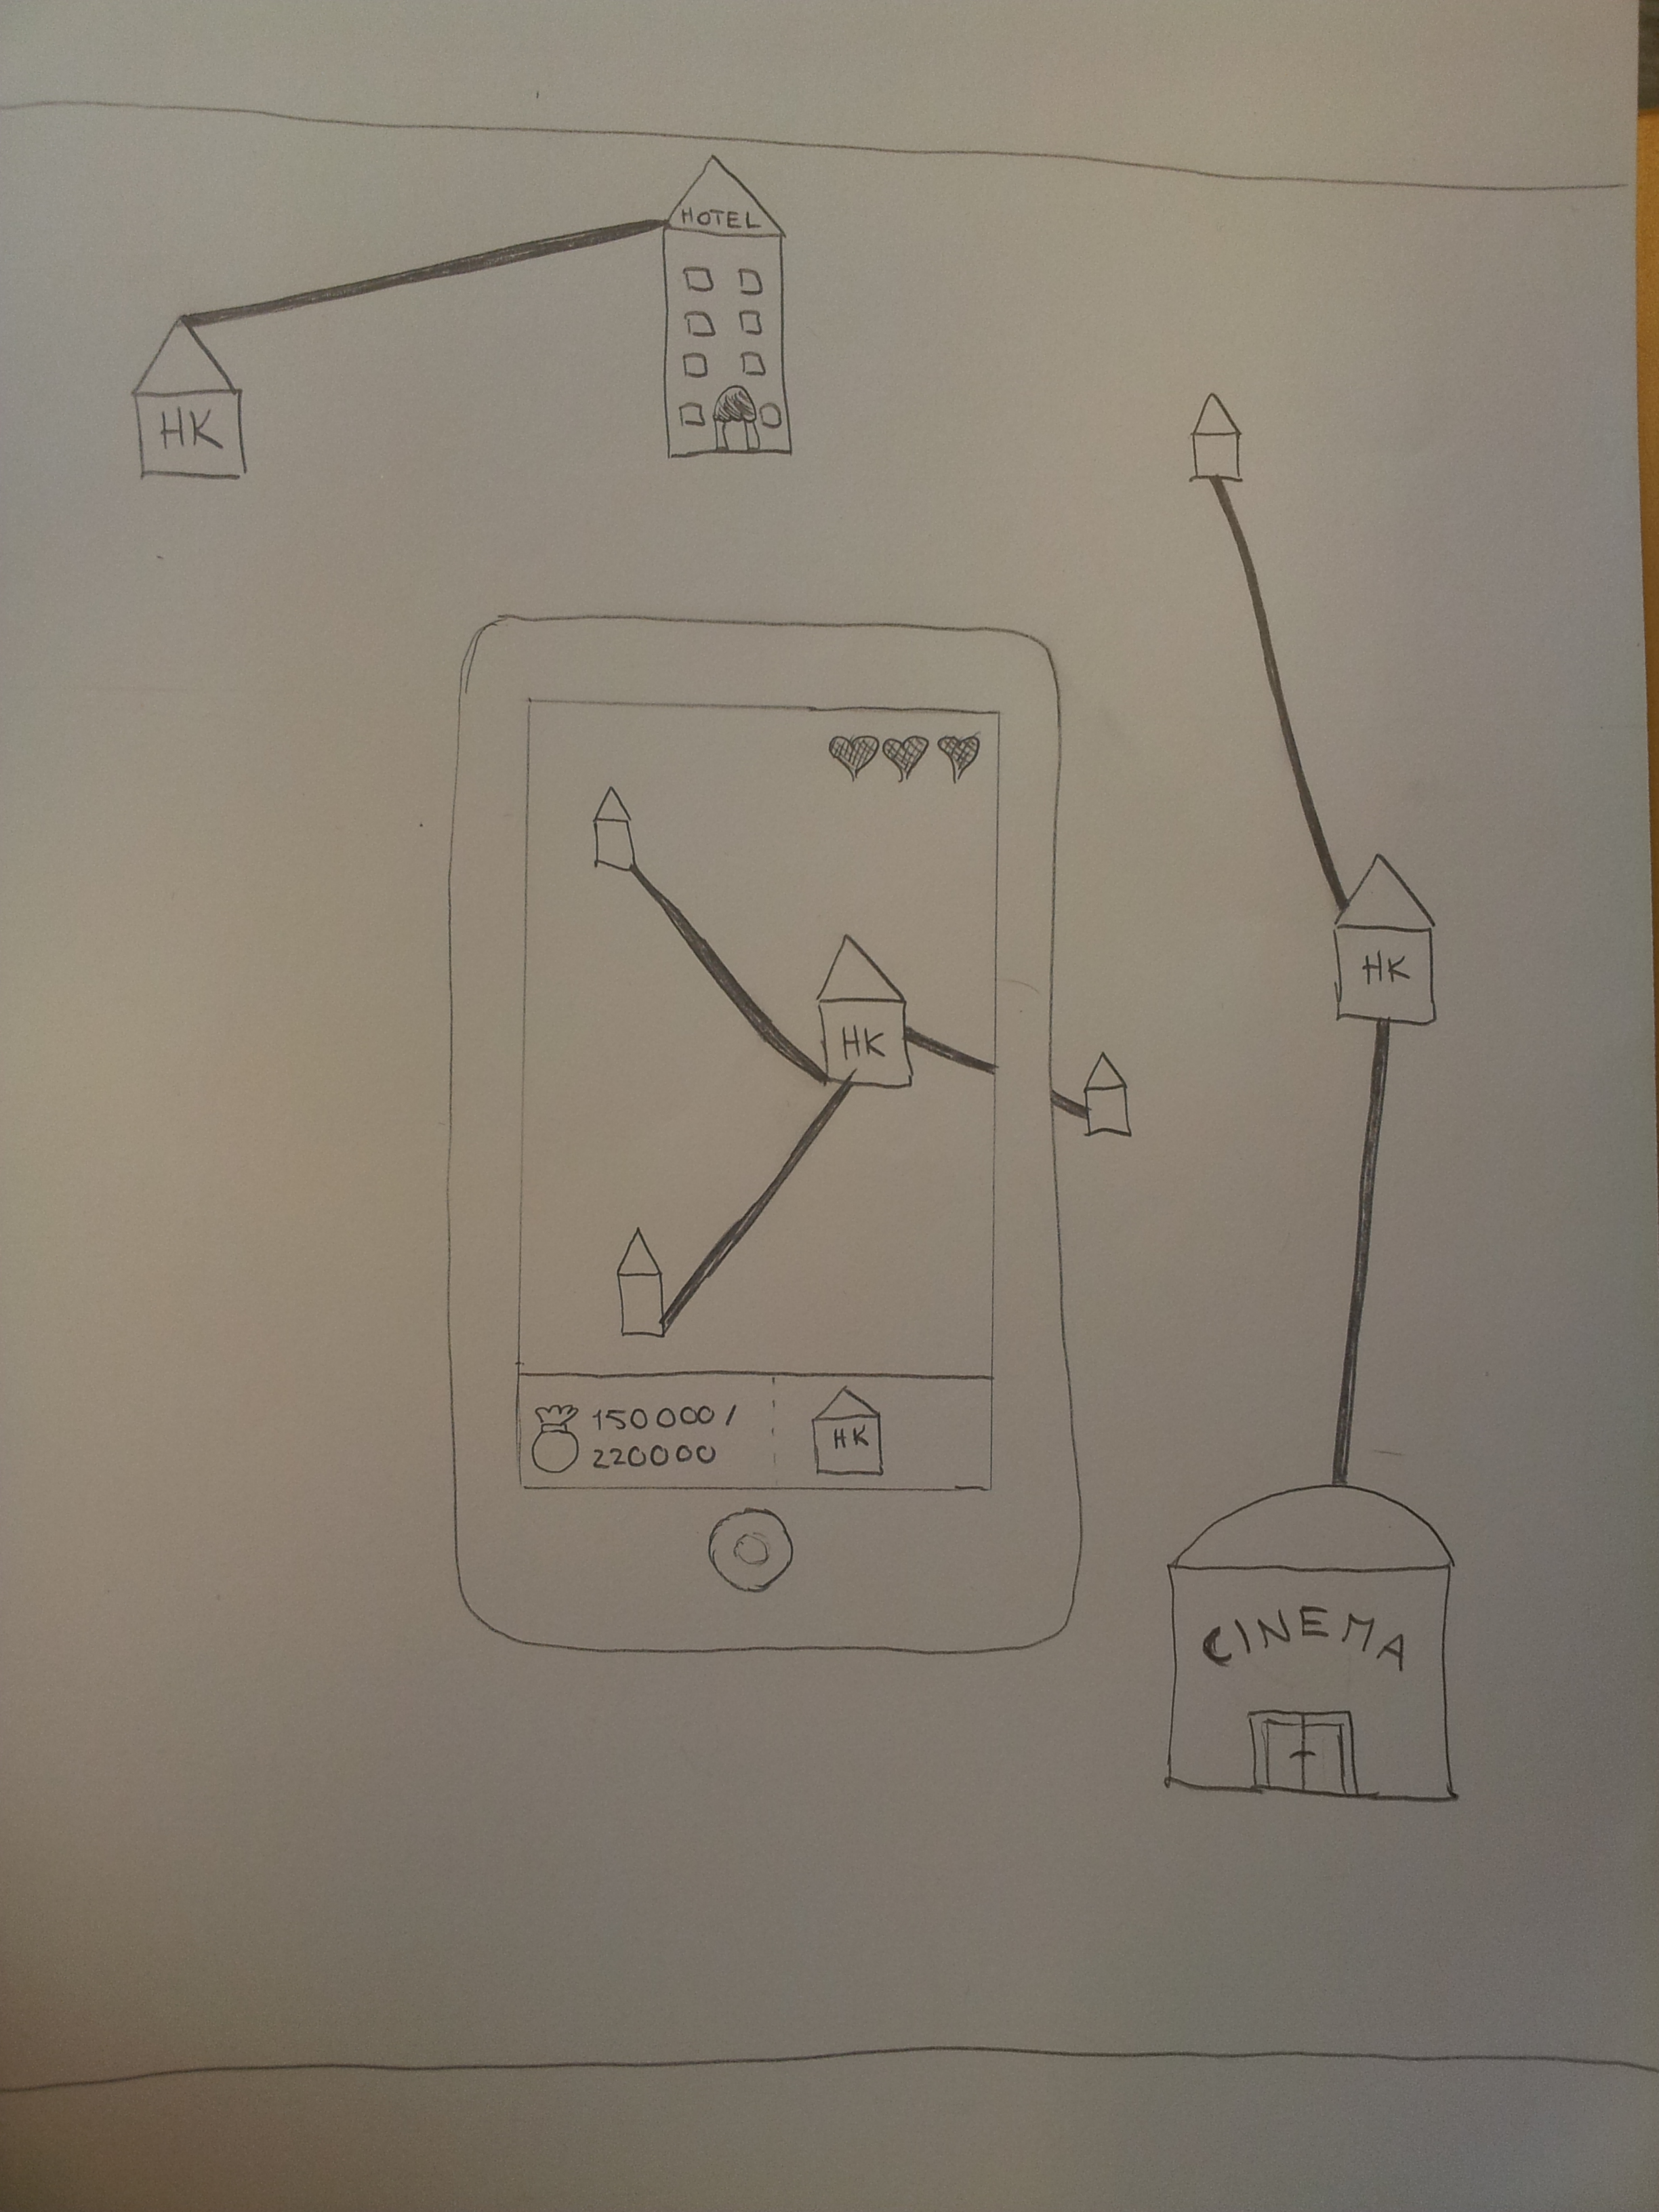
\includegraphics[scale=0.05]{pictures/gameConcept2}
		}
	\end{figure}

\subsection{Specification of the Requirements}
	After the group had finished the game concept and the customer approved the concept the
	focus was to get a clear list of requirements for the game. The list of requirements 
	(the requirement specification) needs a signature from the customer in order to be able
	to give a impression of what the customer can expect at the final delivery.

	The requirement specification consists of functional and non-functional requirements to
	fullfill in the project. All the functional requirements have a priority as well as a 
	conplexity factor assigned. When we made the requirement specification, we made it quite 
	ambitious. The requirements are reqistered with a priority from critical to low. We have
	talked to the customer with a notification that we might not get the time to implement all
	of the requirements, but we will implement them in the order from critical to low. 

\subsection{Duration and workload}
	This is the first phase of the project before the sprints are starting. In the start of 
	this phase, scrum master made a template for hour registration that so all the group members
	can register all work done in the project. In each phase we will define activities and each
	person registers hours used on the activity. We add activities as we work. Here is the template 
	that we made:

	\begin{figure}
		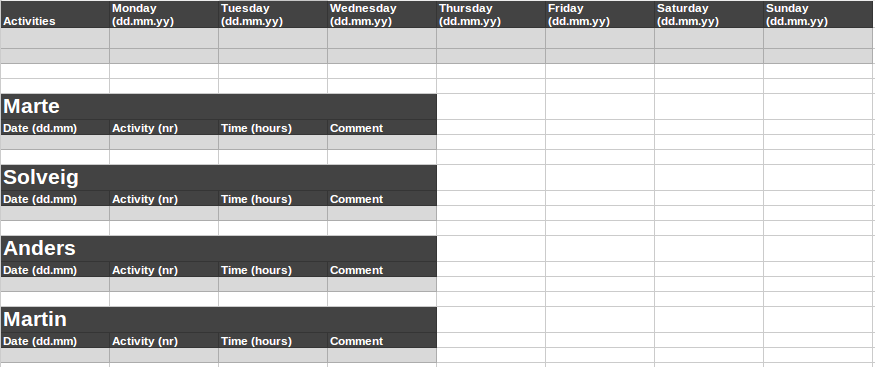
\includegraphics[width=\textwidth]{pictures/timetable.png}
		\caption{Timetable}
	\end{figure}

	In the workload list, the main work was at the planning activity. In this phase we have
	not started any programming, and the development activity is the prestudy for the implementation.

		{\bf Duration:} 09.09 - 29.09 (3 weeks)\\
		{\bf Workload:} This is the list with hours spent (the whole grup) on the project in this sprint.
			\begin{itemize}
				\item {\bf Planning:} 99.5 hours
				\item {\bf Development (prestudy):} 25.5 hours
				\item {\bf Design:} 0 hours
				\item {\bf Documentation (report):} 24.5 hours
				\item {\bf Testing:} 0 hour
			\end{itemize}
		{\bf Total workload: } 149.5 hours \\
	The group's goal was to work at least 20 hours pr/person every week. We did not manage this at this phase, but we had a avrage of 18,7 hours each week pr person (149.5 hours/4 persons/2 weeks = 18.7 hours). 
	The main problem for not working as much as we wanted was because many of the team member has vulentary
	work at organizations as UKA and Abakus. This risk is mentioned in the risk asessment. The group 
	hope to be able to work more the next sprints in order to finish the project and the report at estimated
	time. 

\subsection{Group dynamics}
	When entering the project, non of the group members knew each other, and we used a lot
	of time to know each other better.

	The group work is iniated by the scrum master and the response to discussions are quite low.
	We can see that this can be a problem for the project if the low response in discussions 
	continue in next phases. This is still at a early point in the project and the group might need
	some more time to get the chance to find a good way to work with each other. 
	We have registered the problem and have a dialog with the supervisor about it. 

\subsection{Phase Results}
	In the end of this sprn
